\documentclass[11pt]{article}
\usepackage{amsmath, amssymb}

% Define document version command
\newcommand{\docversion}{v0.2}
\usepackage[a4paper, total={6in, 8in}, margin=0.7in]{geometry}
\usepackage{fancyhdr}
\usepackage{graphicx}
\usepackage{enumitem}
\usepackage{hyperref}
\usepackage{titlesec}
\usepackage{color}
\usepackage{float}

\pagestyle{fancy}
\fancyhf{}
\rhead{ML Technical Interview Notes}
\lhead{Prepared by: DonK}
\rfoot{\thepage}
\lfoot{\docversion}

\title{
  \vspace{1cm}
  \Huge\textbf{ML Technical Interview Prep. Notes} \\
  \vspace{0.5cm}
  \large A Concise Notes for ML Technical Interviews \\
  \vspace{5cm}
  \begin{center}
    
\includegraphics[width=0.7\textwidth]{p_logo.png}
  \end{center}
  \vspace{5cm}
}
\author{\textbf{DonK} \\
\small dongchan@dongchankim.io}
\date{\today}

\begin{document}

% -------------------
% Cover Page
% -------------------
\begin{titlepage}
	\maketitle
	\thispagestyle{empty}
	\vspace*{\fill}
	\small\textit{Note: The order of the questions is categorized by technical topic for clarity.}
\end{titlepage}

% -------------------
% Table of Contents
% -------------------
\pagenumbering{roman}
\tableofcontents
\thispagestyle{empty}
\newpage

% -------------------
% Main Content
% -------------------
\pagenumbering{arabic}

\section{Model Training Fundamentals}

\subsection*{Q: What is the role of Batch Normalization (BN) in training neural networks?}
\textbf{Batch normalization} normalizes the input of each layer to have zero mean and unit variance across a mini-batch. This reduces internal co-variate shift (changes in the distribution of layer inputs during training), speeds up convergence, and stabilizes activation distributions and gradients.

\subsection*{Q: Why are learnable scale and shift parameters (\(\gamma, \beta\)) included in BN?}
BN restricts the distribution of outputs into the same fixed distribution (mean=0, variance=1), which prevents the network from learning the optimal scale and bias. These parameters allow the network to undo the normalization if necessary, preserving representational power after the input is normalized.

\subsection*{Q: Where should BN be applied in a neural network?}
\textbf{Batch normalization} is typically applied after the affine transformation (like a linear or convolutional layer) and before the activation function such as ReLU. BN normalizes the pre-activation values which stabilizes the distribution before they pass through nonlinearities, which keeps gradients flowing smoothly during backpropagation. BN, typically, is not applied to the output layers.

\subsection*{Q: What are the limitations of BN with small batch sizes?}
Small batch sizes lead to noisy estimates of the mean and variance, which can destabilize training and degrade performance. This may result in issues such as batch-wise overfitting or jittery parameter updates. Additionally, Batch Normalization loses much of its regularization effect when batch statistics become unreliable. In practice, a "small batch" typically refers to fewer than 32 samples per batch per device.

\subsection*{Q: How does batch normalization work during inference?}
During inference, batch normalization (BN) uses the running averages of the mean and variance computed during training, rather than calculating them from the current batch of data. This ensures deterministic outputs regardless of batch size. However, the outputs during inference may differ slightly from those during training due to the shift from batch-wise statistics to running estimates.

\subsection*{Q: How do BatchNorm, LayerNorm, GroupNorm, and InstanceNorm compare?}
\begin{figure}[H]
	\centering
	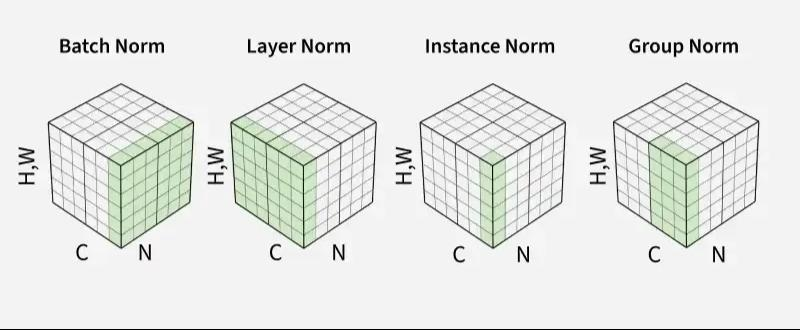
\includegraphics[width=0.8\textwidth]{norms.jpg}
	\caption{Source: \textit{https://www.geeksforgeeks.org/deep-learning/what-is-group-normalization/}}
\end{figure}
\begin{itemize}
	\item \textbf{Batch Normalization (BatchNorm)}: BatchNorm normalizes inputs across the batch dimension for each feature channel. It works well with large batch sizes and helps stabilize and accelerate training, but it can perform poorly with small batches and behaves differently during inference.
	\item \textbf{Layer Normalization (LayerNorm)}: LayerNorm normalizes across all feature dimensions within a single data sample. It is independent of batch size (robust for small batches) and is commonly used in architectures like Transformers and RNNs, but it tends to be less effective in convolutional neural networks.
	\item \textbf{Group Normalization (GroupNorm)}: GroupNorm divides channels into smaller groups and normalizes within each group. It performs consistently regardless of batch size and is particularly effective for convolutional models, though it requires tuning the number of groups (e.g., num groups=32).
	\item \textbf{Instance Normalization (InstanceNorm)}: InstanceNorm normalizes each individual sample and channel across spatial dimensions. It is widely used in style transfer applications as it helps remove instance-specific contrast information, but it may hurt performance in classification tasks where style information is important.
\end{itemize}

In summary, the choice of normalization method depends heavily on the task and batch size. For convolutional neural networks (CNNs) trained on large datasets like ImageNet, \textbf{BatchNorm} is the preferred choice. In scenarios with small batch sizes, such as object detection or segmentation, \textbf{GroupNorm} is typically more stable and effective. For natural language processing (NLP) and Transformer-based architectures, \textbf{LayerNorm} is widely used due to its batch-size independence. Finally, in style transfer or generative adversarial networks (GANs), \textbf{InstanceNorm} is favored for its ability to discard contrast and style-specific information.

\subsection*{Q: What is a feature and what is a channel in the context of machine learning and deep learning?}
\begin{itemize}
	\item A \textbf{feature} generally refers to an individual, measurable property or characteristic extracted from raw data. Features serve as input signals that help a machine learning model learn patterns and make predictions or decisions.

	\item A \textbf{channel}, in the context of deep learning—particularly convolutional neural networks (CNNs)—refers to the depth dimension of the input or output tensor. It corresponds to the number of filters or feature maps learned by a convolutional layer. For example, an RGB image has three channels (red, green, blue), and a CNN may produce dozens or hundreds of channels after processing.
\end{itemize}

\section{Optimization Algorithms}

\subsection*{Q: What are the differences between SGD and Adam?}
\textbf{SGD} uses a fixed or scheduled learning rate and is memory-efficient. \textbf{Adam} adapts learning rates for each parameter and converges faster but may overfit.

\subsection*{Q: What is the role of momentum in SGD?}
\textbf{Momentum} accumulates past gradients to smooth updates and accelerate convergence, especially in consistent gradient directions, and dampen oscillations caused by noisy gradients.

\section{Regularization Techniques}

\subsection*{Q: How can overfitting be reduced in machine learning models?}
Techniques include collecting more data (e.g., data augmentation), regularization (e.g., weight decay, dropout, L1/L2 regularization), early stopping, learning rate scheduling, model simplification, and model ensembling.

\subsection*{Q: What is the difference between L1 and L2 regularization?}
\textbf{L1} adds absolute value penalties, leading to sparse models. \textbf{L2} adds squared penalties, keeping weights small but non-zero.

\subsection*{Q: How does dropout work?}
\textbf{Dropout} is a regularization technique that randomly deactivates (or "drops") neurons during training with a specified probability. This prevents the network from becoming overly reliant on specific neurons and encourages redundancy in learned representations, which helps reduce overfitting.

A high dropout rate increases regularization, which may cause the model to underfit if too much information is lost. Conversely, a low dropout rate provides weaker regularization, which may lead to overfitting if the model memorizes training data.

\subsection*{Q: Why does dropout improve generalization?}
\textbf{Dropout} acts like training many sub-networks and adds noise to the training process, which reduces overfitting and improves generalization.

\section{Loss Functions and Evaluation}

\subsection*{Q: What are commonly used loss functions in ML?}
Commonly used loss functions in machine learning include the following:
\begin{itemize}
	\item \textbf{Mean Squared Error (MSE)} is used in regression tasks and penalizes the squared difference between predicted and actual values.
	      \[
		      \mathcal{L}_{\text{MSE}} = \frac{1}{n} \sum_{i=1}^{n} (y_i - \hat{y}_i)^2
	      \]

	\item \textbf{Binary Cross Entropy (BCE)} is used for binary classification and measures the difference between predicted probabilities and true binary labels.
	      \[
		      \mathcal{L}_{\text{BCE}} = - \frac{1}{n} \sum_{i=1}^{n} \left[ y_i \log(\hat{y}_i) + (1 - y_i) \log(1 - \hat{y}_i) \right]
	      \]

	\item \textbf{Cross-Entropy Loss} is applied in multi-class classification problems to quantify the divergence between predicted class probabilities and the actual class label.
	      \[
		      \mathcal{L}_{\text{CE}} = - \sum_{i=1}^{n} \sum_{c=1}^{C} y_{i,c} \log(\hat{y}_{i,c})
	      \]
	      where \( C \) is the number of classes, \( y_{i,c} \in \{0,1\} \) is the true label, and \( \hat{y}_{i,c} \) is the predicted probability for class \( c \).

	\item \textbf{Hinge Loss}, leading to the canonical Support Vector Machines (SVMs), promotes a margin between classes to improve classification confidence.
	      \[
		      \mathcal{L}_{\text{Hinge}} = \frac{1}{n} \sum_{i=1}^{n} \max(0, 1 - y_i \hat{y}_i)
	      \]
	      where \( y_i \in \{-1, 1\} \) is the true class label, and \( \hat{y}_i \) is the predicted score.
\end{itemize}

\subsection*{Q: What is a ROC curve and what does AUC represent?}
\textbf{ROC (Receiver Operating Characteristic) curve} illustrates the trade-off between the True Positive Rate (TPR, also known as recall) and the False Positive Rate (FPR) across various classification thresholds. It visualizes how well a binary classifier can distinguish between positive and negative classes at different decision boundaries. \\
\textbf{AUC (Area Under the Curve)} is a scalar value that summarizes the overall performance of the model. It represents the probability that a randomly chosen positive example is ranked higher than a randomly chosen negative one. Interpretation of AUC values:
\begin{itemize}
	\item \textbf{1.0} — Perfect classification
	\item \textbf{0.9–1.0} — Excellent performance
	\item \textbf{0.8–0.9} — Good performance
	\item \textbf{0.7–0.8} — Acceptable performance
	\item \textbf{0.5} — No better than random guessing
	\item \textbf{$<$ 0.5} — Worse than random (indicates a potential label inversion)
\end{itemize}

\subsection*{Q: What is a ROC curve and what does AUC represent?}
\textbf{ROC (Receiver Operating Characteristic) curve} illustrates the trade-off between the True Positive Rate (TPR, also known as recall) and the False Positive Rate (FPR) across various classification thresholds. It visualizes how well a binary classifier can distinguish between positive and negative classes at different decision boundaries.

\[
	\text{TPR} = \frac{\text{TP}}{\text{TP} + \text{FN}} \quad \text{(True Positive Rate)}, \quad
	\text{FPR} = \frac{\text{FP}}{\text{FP} + \text{TN}} \quad \text{(False Positive Rate)}
\]

Each point on the ROC curve corresponds to a different threshold used to convert predicted probabilities into class labels. \\ \\
\textbf{AUC (Area Under the Curve)} is a scalar value that summarizes the overall performance of the model. It represents the probability that a randomly chosen positive example is ranked higher than a randomly chosen negative one.

\[
	\text{AUC} = \int_{0}^{1} \text{TPR}(\text{FPR}) \, d(\text{FPR})
\]
\\
Interpretation of AUC values:
\begin{itemize}
	\item \textbf{1.0} — Perfect classification
	\item \textbf{0.9–1.0} — Excellent performance
	\item \textbf{0.8–0.9} — Good performance
	\item \textbf{0.7–0.8} — Acceptable performance
	\item \textbf{0.5} — No better than random guessing
	\item \textbf{$<$ 0.5} — Worse than random (indicates a potential label inversion)
\end{itemize}

\section{Model Architectures}

\subsection*{Q: How do Transformers differ from traditional Seq2Seq models?}
\textbf{Transformers} use self-attention instead of recurrence, enabling parallelism and better modeling of long-range dependencies by self-attention and positional embeddings.

\subsection*{Q: What are positional embeddings and why are they used in Transformers?}
\textbf{Positional embeddings} encode token positions, which allows the transformer to maintain sequence order since self-attention lacks inherently order awareness, otherwise.

\subsection*{Q: What are common activation functions and their pros/cons?}
\begin{figure}[H]
	\centering
	\includegraphics[width=0.8\textwidth]{activation.png}
	\caption{Source: \textit{https://blog.devops.dev/exploring-activation-functions-in-deep-learning-properties-derivatives-and-impact-on-model-7585aad8a757}.}
\end{figure}

\begin{itemize}
	\item \textbf{Sigmoid}: The sigmoid function is easy to interpret as it outputs values in (0, 1), but it may suffer from the vanishing gradient problem, especially at extreme input values.
	      \[
		      \sigma(x) = \frac{1}{1 + e^{-x}}
	      \]

	\item \textbf{Tanh}: The tanh function is zero-centered and ranges (-1, 1), which can help with optimization, but like the sigmoid function, it also experiences vanishing gradients.
	      \[
		      \tanh(x) = \frac{e^x - e^{-x}}{e^x + e^{-x}}
	      \]

	\item \textbf{ReLU}: The ReLU (Rectified Linear Unit) function is computationally efficient and helps create sparse representations, but it can suffer from the "dying ReLU" problem, where neurons become inactive.
	      \[
		      \text{ReLU}(x) = \max(0, x)
	      \]

	\item \textbf{Leaky ReLU}: The Leaky ReLU addresses the dying ReLU issue by allowing a small, non-zero gradient when the unit is not active, improving learning stability.
	      \[
		      \text{LeakyReLU}(x) =
		      \begin{cases}
			      x        & \text{if } x \geq 0 \\
			      \alpha x & \text{if } x < 0
		      \end{cases}
	      \]
	      where \( \alpha \) is a small positive constant (typically \( \alpha = 0.01 \)).

	\item \textbf{Softmax}: The softmax function converts logits into a probability distribution over classes, making it suitable for multi-class classification problems.
	      \[
		      \text{Softmax}(z_i) = \frac{e^{z_i}}{\sum_{j=1}^{C} e^{z_j}}
	      \]
	      where \( z_i \) is the logit for class \( i \), and \( C \) is the number of classes.
\end{itemize}

\subsection*{Q: When should you use Sigmoid vs Softmax?}
Use Sigmoid for binary or multi-label tasks. Use Softmax for mutually exclusive multi-class classification.

\subsection*{Q: What is Byte Pair Encoding (BPE) and why is it used?}
\textbf{Byte Pair Encoding (BPE)} is a subword tokenization algorithm that decomposes text into units that strike a balance between individual characters and complete words. It begins by treating each character as a separate token and then iteratively merges the most frequent adjacent pairs of tokens into new combined tokens. This approach improves model performance by:
\begin{itemize}
	\item reducing the overall vocabulary size
	\item handling out-of-vocabulary words effectively
	\item improving tokenization efficiency
\end{itemize}

BPE is widely used in modern language models such as GPT and RoBERTa due to its ability to efficiently tokenize large corpora while preserving useful linguistic structures.

\subsection*{Q: What are the common decoding techniques used in large language models (LLMs)?}
Several decoding techniques are used to generate text from large language models, each with different trade-offs between determinism, diversity, and coherence:

\begin{itemize}
	\item \textbf{Greedy Decoding}: This method selects the token with the highest probability at each step. While it is fast and deterministic, it often produces repetitive or suboptimal outputs because it doesn't explore alternative paths.
	\item \textbf{Beam Search}: Beam search keeps track of the top \(k\) most probable sequences (beams) at each decoding step and expands them in parallel. It balances quality and computation by considering multiple candidates, but it can still produce generic responses and is less diverse than sampling-based methods.
	\item \textbf{Top-\(k\) Sampling}: Instead of always choosing the most likely token, top-\(k\) sampling samples from the top \(k\) most probable next tokens. This introduces randomness and improves diversity, making outputs more creative and less deterministic.
	\item \textbf{Top-\(p\) Sampling (Nucleus Sampling)}: This method selects from the smallest possible set of tokens whose cumulative probability exceeds a threshold \(p\) (e.g., 0.9). It adapts the candidate pool dynamically and often results in more coherent yet diverse outputs compared to top-\(k\) sampling.
	\item \textbf{Temperature Scaling}: Although not a decoding method itself, temperature is a parameter often used during sampling to control randomness. A lower temperature makes the model more confident (peaky distributions), while a higher temperature makes it more random and exploratory.
\end{itemize}

\subsection*{Q: What is MMOE and what are some other multi-objective learning algorithms?}
\begin{itemize}
	\item \textbf{MMOE (Multi-gate Mixture-of-Experts)} is a neural network architecture designed for multi-task learning, where a single model simultaneously learns to perform multiple related tasks. MMOE consists of:
	      \begin{itemize}
		      \item A set of shared \textbf{experts} (typically fully connected networks) that learn general-purpose representations.
		      \item A set of task-specific \textbf{gating networks} that learn how to combine the outputs of the shared experts differently for each task.
	      \end{itemize}
	      This design allows the model to balance shared and task-specific information, improving performance and reducing negative transfer between tasks.

	\item \textbf{Cross-Stitch Networks}: These networks allow linear combinations of activations from task-specific models. The model learns how much information to share at each layer between tasks by learning cross-stitch units.

	\item \textbf{Shared Bottom + Task-Specific Heads}: This is a simple and widely used approach where early layers are shared among tasks to extract common features, while the top layers (heads) are task-specific to capture task-dependent patterns.

	\item \textbf{PLE (Progressive Layered Extraction)}: PLE introduces shared and task-specific experts at multiple levels and progressively separates representations using gating networks, enhancing performance in complex multi-task scenarios.

	\item \textbf{PCGrad (Projected Gradient Descent)}: PCGrad is an optimization-based method for multi-objective learning. It resolves gradient conflicts between tasks by projecting conflicting gradients onto each other’s normal planes, avoiding destructive interference during learning.

	\item \textbf{GradNorm}: This algorithm dynamically balances the training of multiple tasks by adjusting the gradients' magnitudes to ensure that all tasks train at a similar rate, preventing task dominance.

\end{itemize}

Multi-objective and multi-task learning algorithms are especially useful when tasks are related and can benefit from shared representations, improving generalization and model efficiency.


\section{Fine-Tuning Techniques}

\subsection*{Q: What is PEFT (Parameter-Efficient Fine-Tuning)?}
\textbf{PEFT} fine-tunes only a subset of parameters, reducing memory and compute costs while preserving performance.

\subsection*{Q: What is LoRA and how does it work?}
\textbf{LoRA} adds low-rank trainable matrices to frozen layers, reducing the number of trainable parameters for speed and memory-efficiency.

\subsection*{Q: What is QLoRA and why is it useful?}
\textbf{QLoRA} applies LoRA to the quantized models (e.g., 4-bit), enabling fine-tuning of large models on limited hardware. Once all the training is done, the original weights will be de-quantized.

\section{Fundamental ML Concepts}

\subsection*{Q: What is the difference between MLE and MAP estimation?}
\textbf{MLE} maximizes the likelihood of observing the given data. \textbf{MAP} includes priors to maximize posterior probability.

\subsection*{Q: What is the difference between generative and discriminative models?}
\textbf{Generative models} model the joint probability, \(P(x, y)\), to generate data. \textbf{Discriminative models} the conditional probability, \(P(y|x)\), to distinguish classes.

\subsection*{Q: What is the bias-variance tradeoff in machine learning?}
\begin{itemize}
	\item \textbf{Bias} refers to the model's specificity, introduced by approximating a complex problem using a simplified model. High bias can cause a model to miss relevant patterns in the data, leading to underfitting.
	\item \textbf{Variance} refers to the model's sensitivity (recall) to small fluctuations in the training data. A high-variance model captures noise along with the signal, leading to overfitting.
	\item A model with high bias and low variance is too simple to capture the underlying structure of the data (underfitting), whereas a model with low bias and high variance captures noise and fails to generalize well (overfitting).
\end{itemize}

\section{Recommender Systems}

\subsection*{Q: What is collaborative filtering and what are its types?}
\textbf{Collaborative filtering} recommends items based on user/item similarity. Types include user-based, item-based, and matrix factorization.

\subsection*{Q: What are the limitations of collaborative filtering?}
\begin{itemize}
	\item \textbf{Cold-start problem}: Collaborative filtering requires a history of user-item interactions to make recommendations. When new users or items enter the system, the lack of historical data makes it difficult to generate accurate recommendations.
	\item \textbf{Data sparsity}: In many real-world applications, users interact with only a small fraction of available items, leading to a sparse user-item matrix. This sparsity reduces the effectiveness of similarity-based methods and can negatively impact the quality of recommendations.
	\item \textbf{Scalability}: As the number of users and items grows, computing similarity scores and performing matrix factorization becomes computationally expensive, posing challenges for real-time recommendation at scale.
	\item \textbf{Popularity bias}: Collaborative filtering tends to recommend popular items more frequently, which can lead to a lack of diversity in recommendations and overlook niche or less-rated content.
	\item \textbf{Lack of contextual understanding}: Collaborative filtering does not typically incorporate side information such as time, location, or user demographics, which may be crucial for making context-aware recommendations.
\end{itemize}

\subsection*{Q: What is the two-tower model?}
The \textbf{two-tower model} is a neural architecture commonly used for tasks like recommendation, retrieval, and matching. It consists of two separate neural networks (or “towers”)—one for encoding the query (e.g., user, question, search term) and one for encoding the candidate (e.g., item, product, document). Each tower processes its input independently to produce dense vector embeddings.

The similarity between the query and candidate embeddings is then computed—typically using dot product or cosine similarity—to rank or retrieve relevant items. This architecture is efficient for large-scale retrieval since it allows for precomputing and indexing embeddings, enabling fast approximate nearest neighbor (ANN) search.

Key advantages include:
\begin{itemize}
	\item Decoupled processing of queries and items, allowing independent optimization.
	\item Scalability due to efficient embedding retrieval via vector similarity.
	\item Simplicity and interpretability of embedding space.
\end{itemize}

Limitations include:
\begin{itemize}
	\item No cross-interaction between query and item features during encoding.
	\item Suboptimal performance in tasks where joint modeling is important.
\end{itemize}

\subsection*{Q: What are the newer model architectures beyond the two-tower model?}
Several newer architectures have been proposed to address the limitations of the two-tower model, particularly to capture richer interactions between queries and candidates:

\begin{itemize}
	\item \textbf{Cross-Encoder}: Instead of encoding query and candidate separately, a cross-encoder concatenates both inputs and feeds them into a single transformer (e.g., BERT). This allows for deep interaction between inputs and often achieves higher accuracy—but at a much higher computational cost, making it unsuitable for large-scale retrieval.

	\item \textbf{Poly-Encoder}: Proposed by Facebook AI, the poly-encoder balances efficiency and interaction. It uses multiple context vectors (instead of a single one) to attend over the candidate representations. It achieves a middle ground between two-tower and cross-encoder models in terms of performance and speed.

	\item \textbf{ColBERT (Contextualized Late Interaction)}: ColBERT introduces late interaction by computing token-level embeddings using BERT and applying a MaxSim operation across tokens. This allows fine-grained matching while still supporting fast retrieval through ANN techniques.

	\item \textbf{Retriever-Ranker Architecture}: This hybrid approach first uses a fast two-tower retriever to narrow down candidates and then applies a more expressive cross-encoder to re-rank the top candidates. It is widely used in large-scale systems like search engines and QA pipelines.

	\item \textbf{Dense-Sparse Hybrid Models}: Some models combine dense retrieval (like two-tower or ColBERT) with sparse representations (e.g., TF-IDF or BM25) to leverage both semantic similarity and lexical overlap.
\end{itemize}

These newer models improve retrieval accuracy by modeling cross-input interactions, at the cost of increased inference latency and system complexity.

\subsection*{Q: What are common evaluation metrics for recommendation systems?}
Recommendation systems are typically evaluated using metrics that assess ranking quality, relevance, diversity, and user satisfaction. Commonly used evaluation metrics include:

\begin{itemize}
	\item \textbf{Precision@k}: Measures the proportion of relevant items in the top-\(k\) recommended results. It answers: "Out of the top-\(k\) items recommended, how many are relevant?"

	\item \textbf{Recall@k}: Measures the proportion of relevant items that are successfully recommended in the top-\(k\). It answers: "Out of all relevant items, how many were retrieved?"

	\item \textbf{NDCG@k (Normalized Discounted Cumulative Gain)}: Weights the relevance of recommended items based on their position in the ranked list. Higher-ranked relevant items contribute more to the score. This metric reflects the usefulness of the ranking order.

	\item \textbf{Hit Rate@k}: A binary version of recall—it measures whether at least one relevant item appears in the top-\(k\) recommendations.

	\item \textbf{Mean Reciprocal Rank (MRR)}: Computes the reciprocal of the rank of the first relevant item. A higher MRR indicates that relevant items tend to appear earlier in the list.

	\item \textbf{Coverage}: Measures the proportion of all items that the system is capable of recommending. High coverage indicates a broader ability to make diverse recommendations.

	\item \textbf{Diversity and Novelty}: These assess how varied and unexpected the recommendations are. High diversity improves user satisfaction by avoiding redundancy, while novelty introduces users to less familiar content.

	\item \textbf{AUC (Area Under the ROC Curve)}: Measures the probability that a randomly chosen positive item is ranked higher than a randomly chosen negative item. It is used for binary relevance evaluations.

\end{itemize}

Evaluation can be performed in both \textbf{offline} settings (e.g., using historical user-item interactions) and \textbf{online} settings (e.g., through A/B testing and user engagement metrics like click-through rate or dwell time).

\end{document}
